The 95\% confidence level upper limits on the sV and sA model couplings, $\sqrtgqgX$, and the tS model coupling, $\gqX$, which are obtained from each of the \monoX channels, are presented in figs.~ref{}. These quantities were evaluated as described in appendix \ref{AppendixB} and correspond to the best limits of each signal region tested.

In each plot, the grey region represents the phase space where no meaningful limit was obtained, that is, where the limit of at least one of the couplings was found to lie outside the perturbative regime. The white (hatched) regions coincide with those mass points which yield an initial (final) value of $\sqrtgqgX$ which fails to satisfy $\Gamma < \Mmed / 2$. Note that only the \monojet channel produced limits which survive this requirement when $\gX / \gq$ = 0.2, as shown in Fig. \ref{}. We subsequently omit the plots containing the associated limits for the \monoZ and \monoWZ channels.

Some general comments here. Note removal of $\gX / \gq$ = 0.2.

Also, comment about the upper values of coupling - as coupling/4pi becomes closer to 1, perturbativity is failing, as all orders start to become important.

And, the minimum width in the mono-jet t-channel case - this could be larger with the addition of other particles in the larger-scale model, meaning the narrow width effects could disappear. If we are right on the edge of width < M/2, then anything increasing this width would push it over the edge into our non-valid range.

The results are discussed below.

\iffalse
\textcolor{magenta}{This section should include:}
\begin{enumerate}
\item \textcolor{magenta}{Plots for $\sigma(pp \rightarrow X \chi \bar{\chi}$ as a function of $\mX$ for fixed $\Mmed$ and $f$ along with the limits on $f$ using $\sigma \sim f^{4}$.}
\item \textcolor{magenta}{Brief interpretation of the results. I.e. explain "in words" what the plots illustrate.}
\item \textcolor{magenta}{Comparison with previous results (?).}
\end{enumerate}
\fi

\subsection{Mono-jet channel}

Results discussion here.

\subsection{Mono-$Z$ channel}

Mono-Z limits discussion here. Overall uncertainty on $\sqrtgqgX$ generally $ < 10\%$, up to 80$\%$. Large DM masses: small cross sections, limited by ATLAS analysis optimisation, requires more data or further optimisation. Small DM masses: have low $\met$, would require more statistics.

\subsection{Mono-$W/Z$ channel}

Mono-W/Z limits discussion here.
\afterpage{\clearpage}

%\begin{figure}
%  \centering
%  \begin{subfigure}[t]{0.32\textwidth}
%    \centering
%    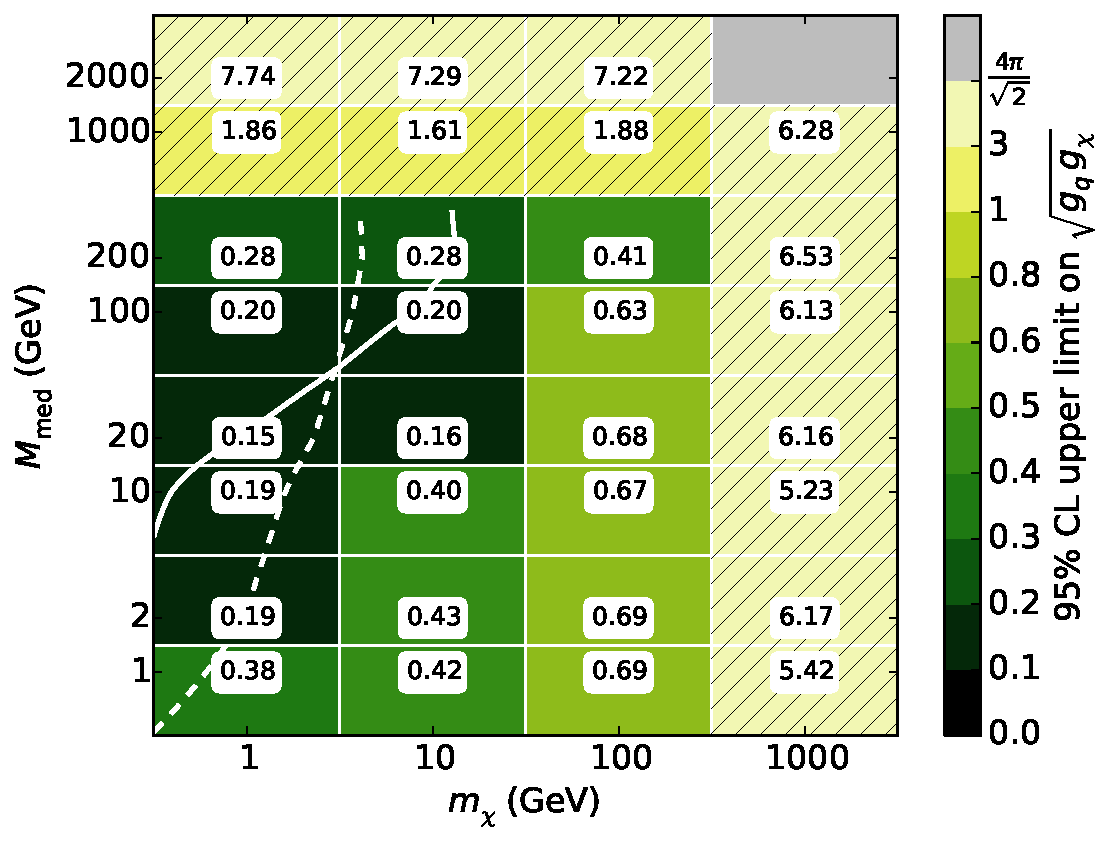
\includegraphics[width=1.\textwidth]{figures/grid_basepoints_SVD_rat05_monojet.pdf}
%    \caption{sV model, $g_q/g_{\chi} = 0.5$, \monojet channel.}
%  \end{subfigure}
%  \caption{}
%\end{figure}

\begin{sidewaysfigure}
  \centering
  \begin{subfigure}[t]{0.32\textwidth}
    \centering
    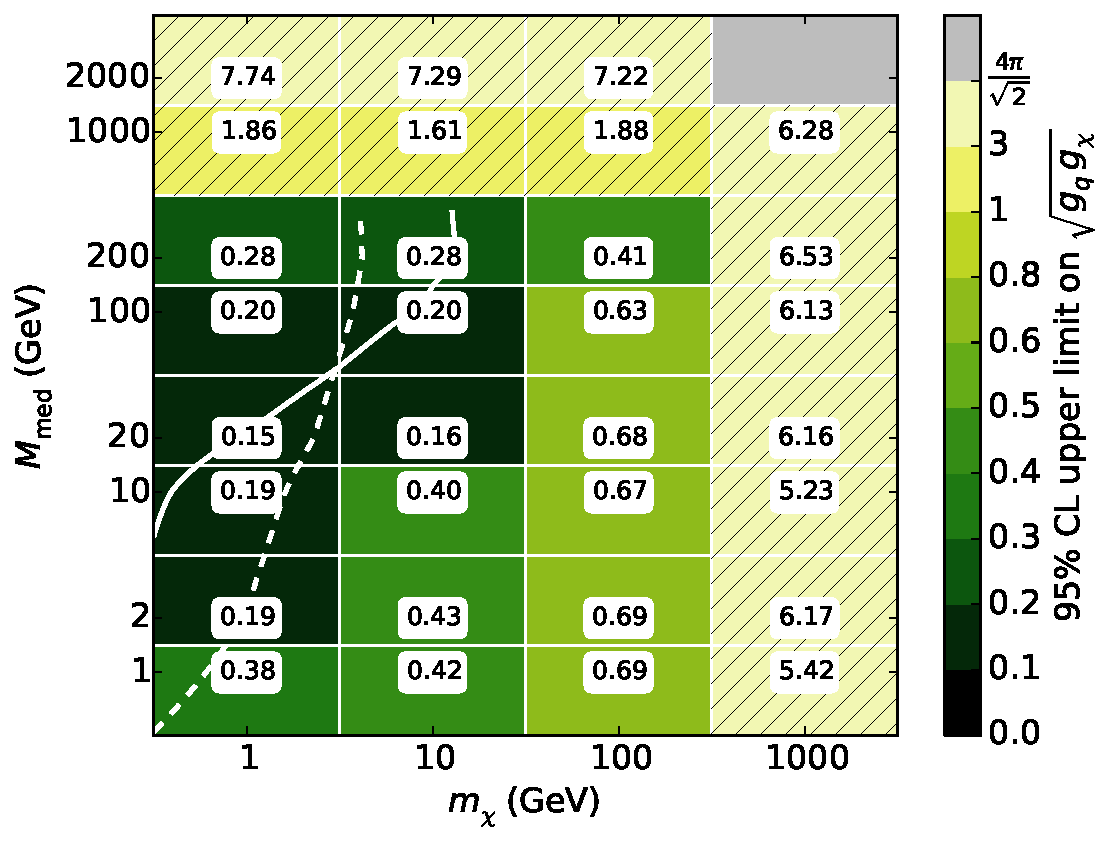
\includegraphics[width=1.\textwidth]{figures/grid_basepoints_SVD_rat05_monojet.pdf}
    \caption{sV model, $g_q/g_{\chi} = 0.5$, \monojet channel.}
  \end{subfigure}
  \begin{subfigure}[t]{0.32\textwidth}
    \centering
    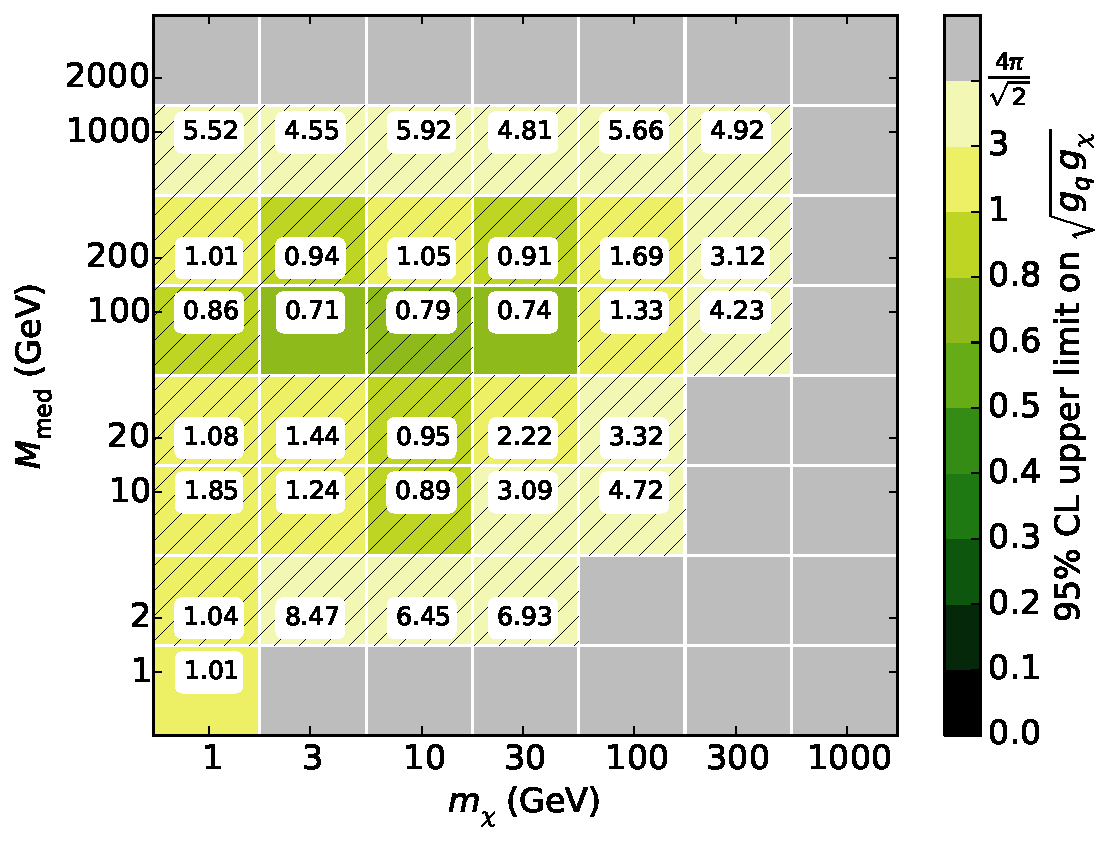
\includegraphics[width=1.\textwidth]{figures/grid_allpoints_SVD_rat05.pdf}
    \caption{sV model, $g_q/g_{\chi} = 0.5$, \monoZ channel.}
  \end{subfigure}
  \begin{subfigure}[t]{0.32\textwidth}
    \centering
    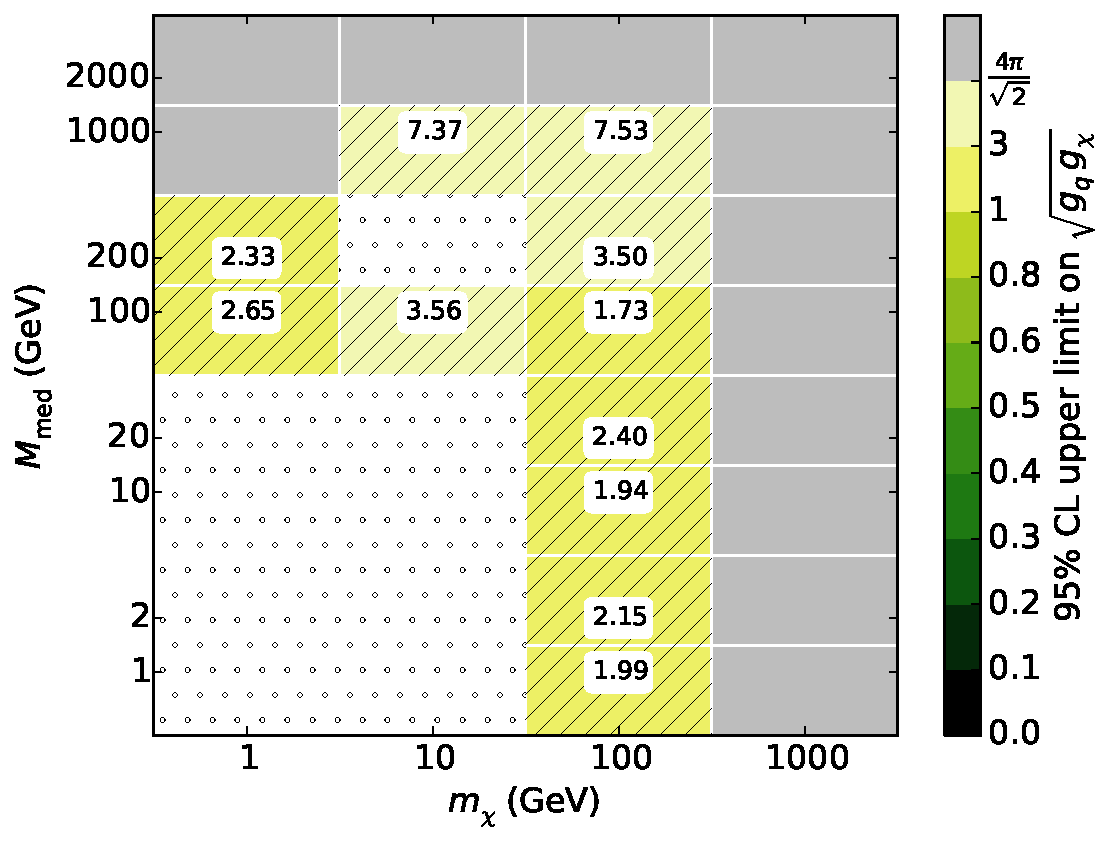
\includegraphics[width=1.\textwidth]{figures/grid_basepoints_SVD_rat05_monoWZ.pdf}
    \caption{sV model, $g_q/g_{\chi} = 0.5$, \monoWZ channel.}
    \vspace{0.75cm}
  \end{subfigure}
  \begin{subfigure}[t]{0.32\textwidth}
    \centering
    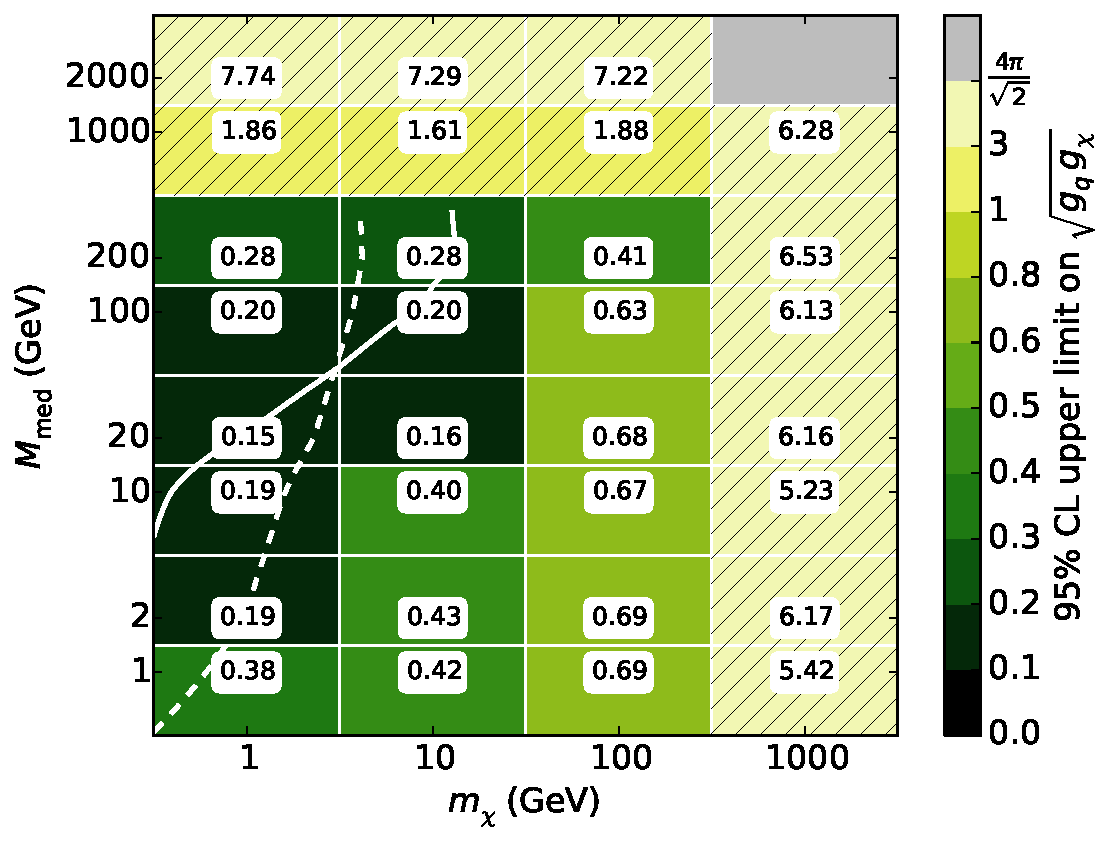
\includegraphics[width=1.\textwidth]{figures/grid_basepoints_SVD_rat05_monojet.pdf} % TODO change to SAD
    \caption{sA model, $g_q/g_{\chi} = 0.5$, \monojet channel.}
  \end{subfigure}
  \begin{subfigure}[t]{0.32\textwidth}
    \centering
    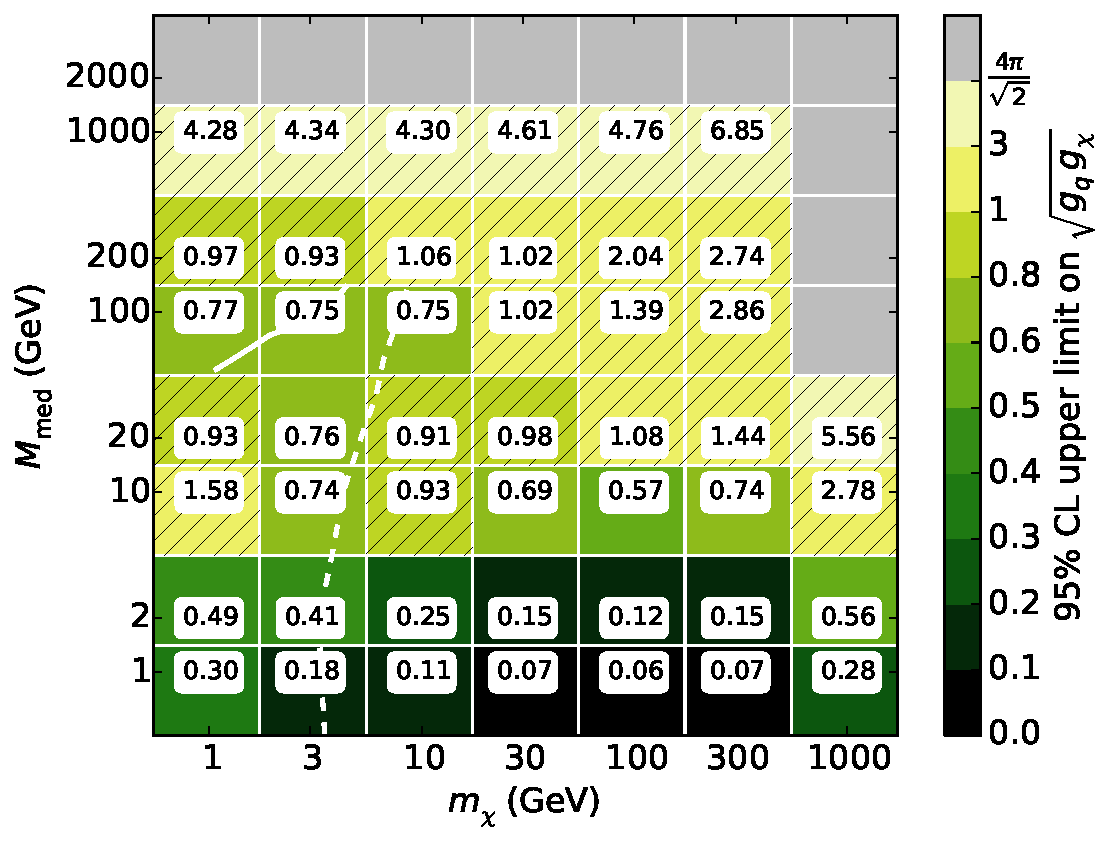
\includegraphics[width=1.\textwidth]{figures/grid_allpoints_SAD_rat05.pdf}
    \caption{sA model, $g_q/g_{\chi} = 0.5$, \monoZ channel.}
  \end{subfigure}
  \begin{subfigure}[t]{0.32\textwidth}
    \centering
    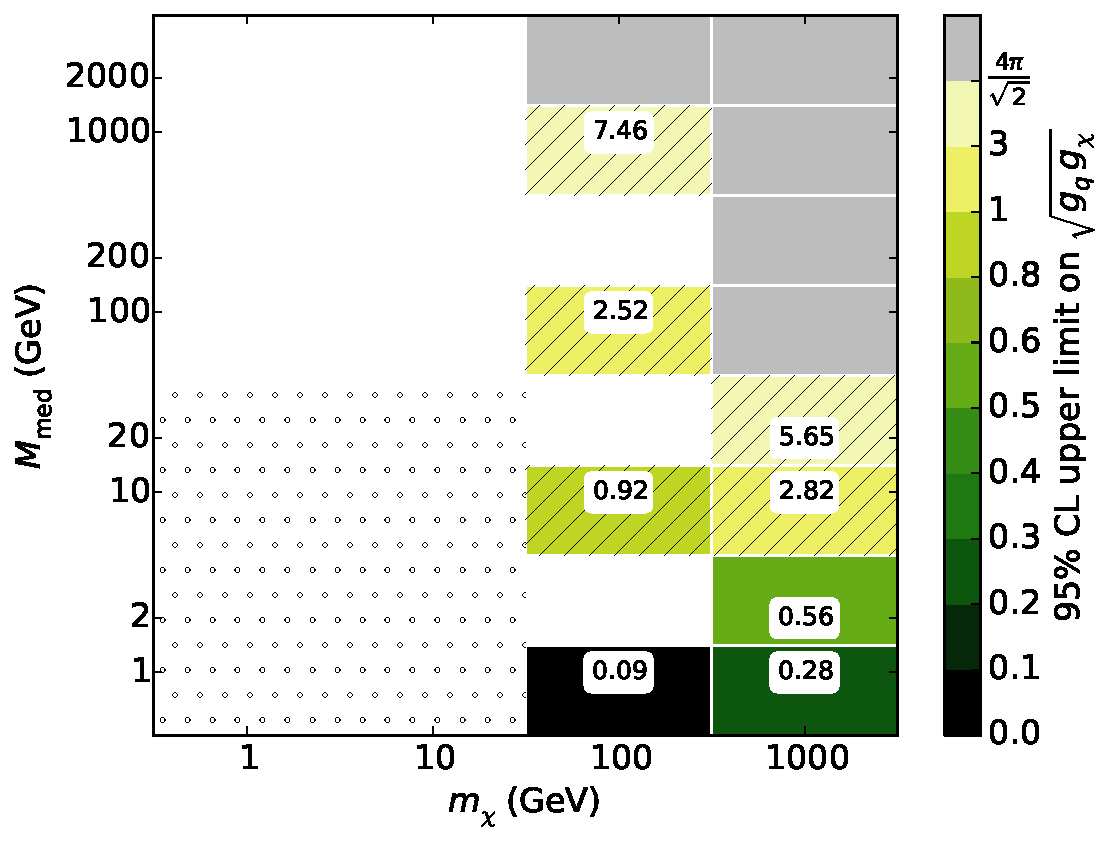
\includegraphics[width=1.\textwidth]{figures/grid_basepoints_SAD_rat05_monoWZ.pdf}
    \caption{sA model, $g_q/g_{\chi} = 0.5$, \monoWZ channel.}
  \end{subfigure}
  \caption{Upper limits on the coupling for the $s$-channel models in the \monojet (left), \monoZ (centre) and \monoWZ (right) channels, for $\gX / \gq$ = 0.5. The grey region represents the phase space where no meaningful limit was obtained. The hatched region represents a limit which leads to a width greater than $\Mmed / 2$, so the validity of the calculation begins to fail. The dotted region represents phase space where insufficient statistics were available.}
  \label{fig:results_sVsA_rat05}
\end{sidewaysfigure}

\begin{sidewaysfigure}
  \centering
  \begin{subfigure}[t]{0.32\textwidth}
    \centering
    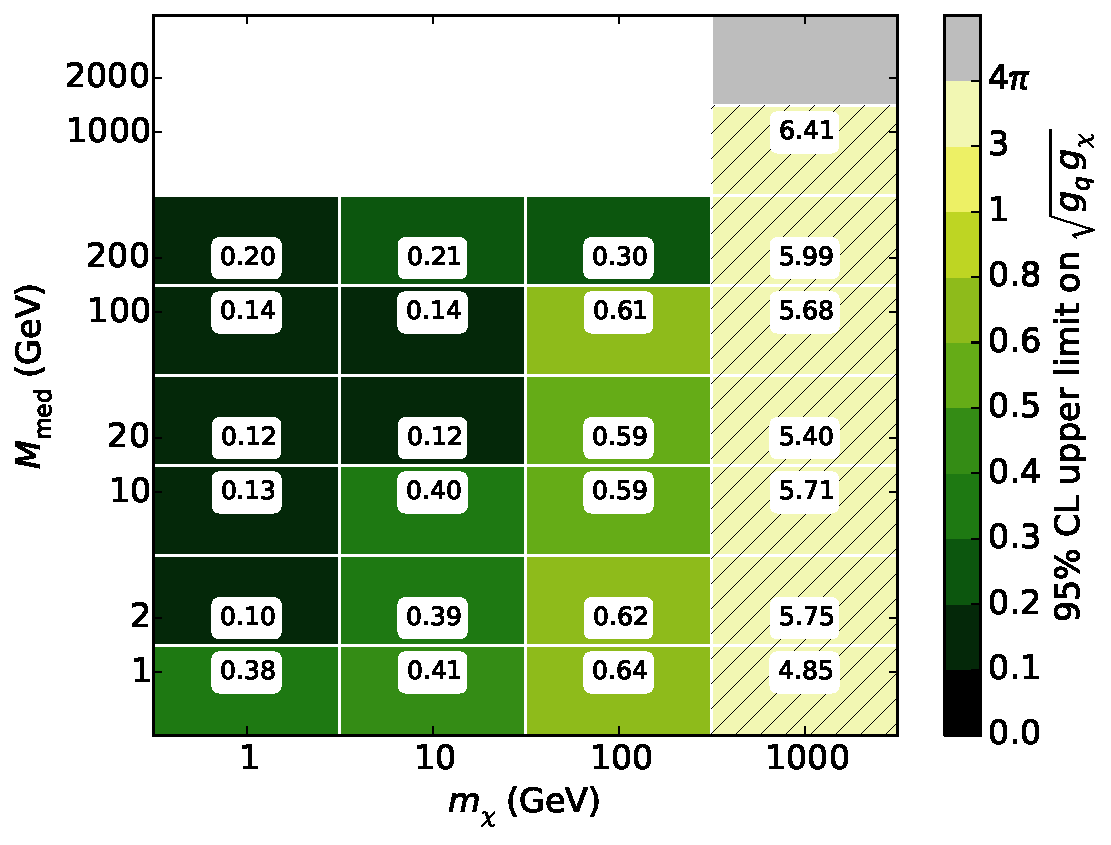
\includegraphics[width=1.\textwidth]{figures/grid_basepoints_SVD_rat1_monojet.pdf}
    \caption{sV model, $g_q/g_{\chi} = 0.5$, \monojet channel.}
  \end{subfigure}
  \begin{subfigure}[t]{0.32\textwidth}
    \centering
    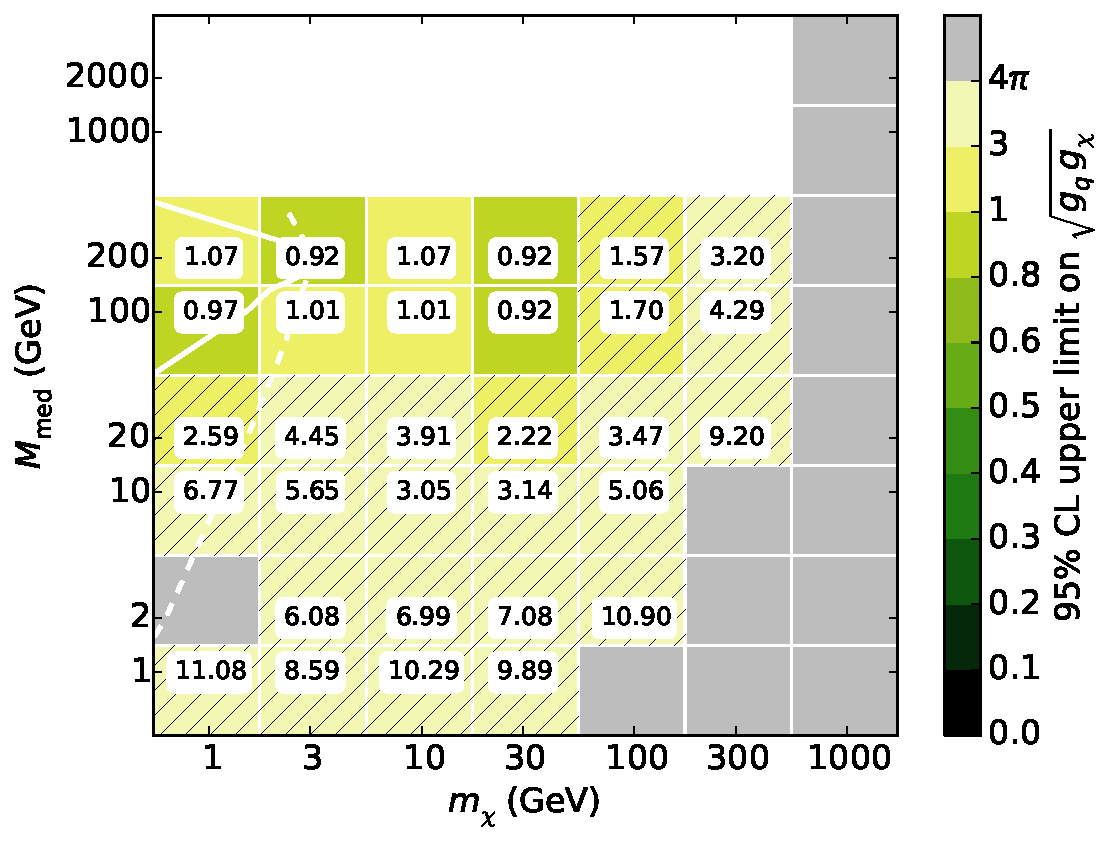
\includegraphics[width=1.\textwidth]{figures/grid_allpoints_SVD_rat1.pdf}
    \caption{sV model, $g_q/g_{\chi} = 0.5$, \monoZ channel.}
  \end{subfigure}
  \begin{subfigure}[t]{0.32\textwidth}
    \centering
    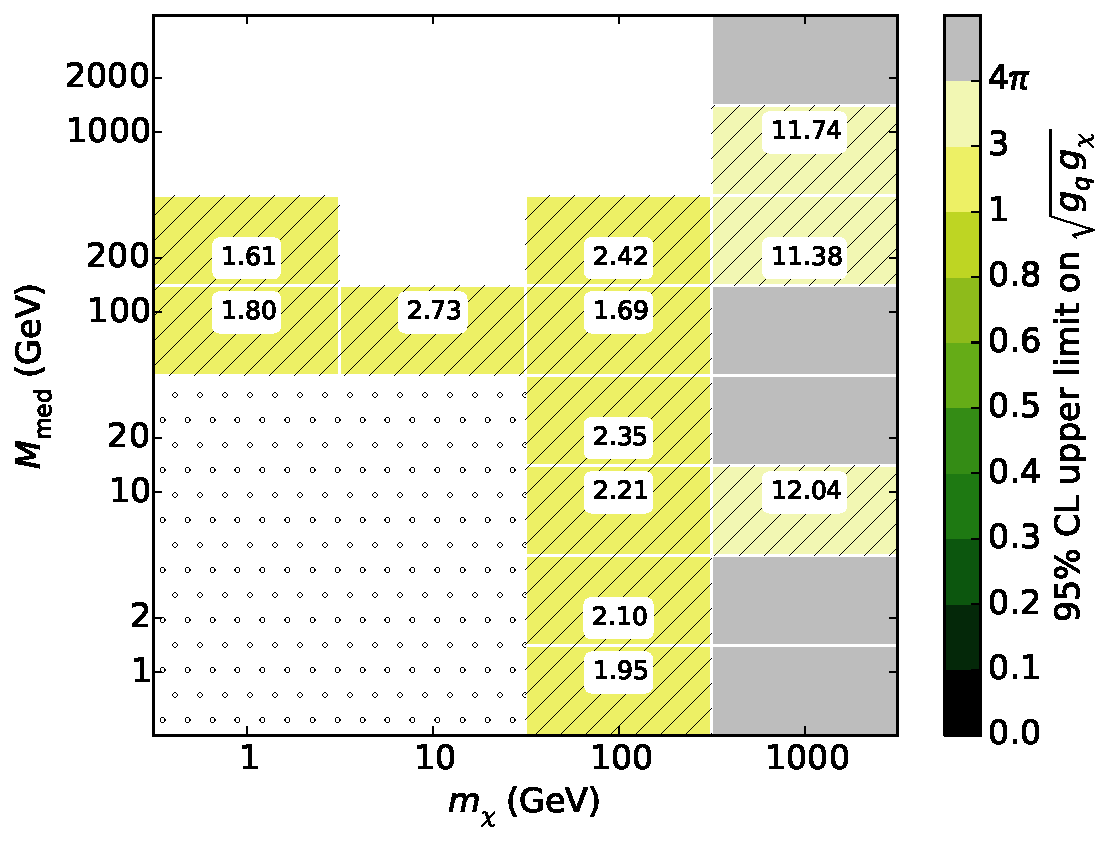
\includegraphics[width=1.\textwidth]{figures/grid_basepoints_SVD_rat1_monoWZ.pdf}
    \caption{sV model, $g_q/g_{\chi} = 0.5$, \monoWZ channel.}
    \vspace{0.75cm}
  \end{subfigure}
  \begin{subfigure}[t]{0.32\textwidth}
    \centering
    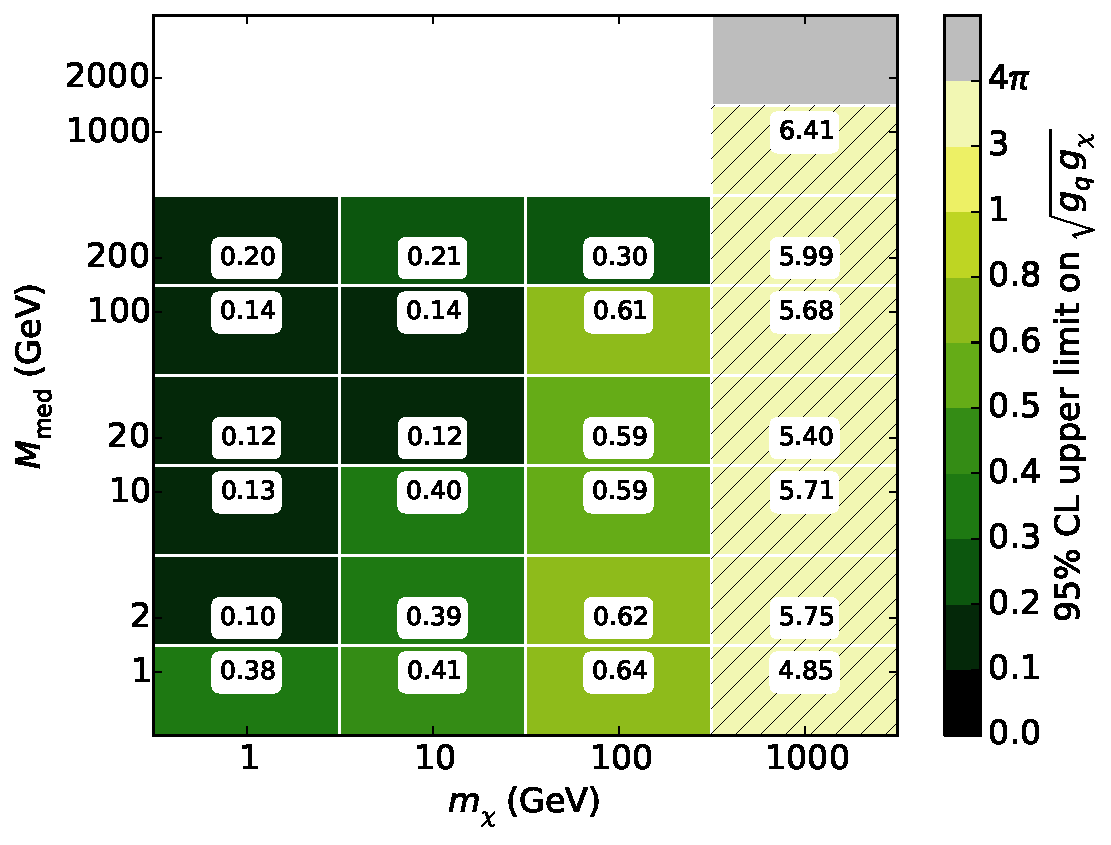
\includegraphics[width=1.\textwidth]{figures/grid_basepoints_SVD_rat1_monojet.pdf}  % TODO change to SAD
    \caption{sA model, $g_q/g_{\chi} = 0.5$, \monojet channel.}
  \end{subfigure}
  \begin{subfigure}[t]{0.32\textwidth}
    \centering
    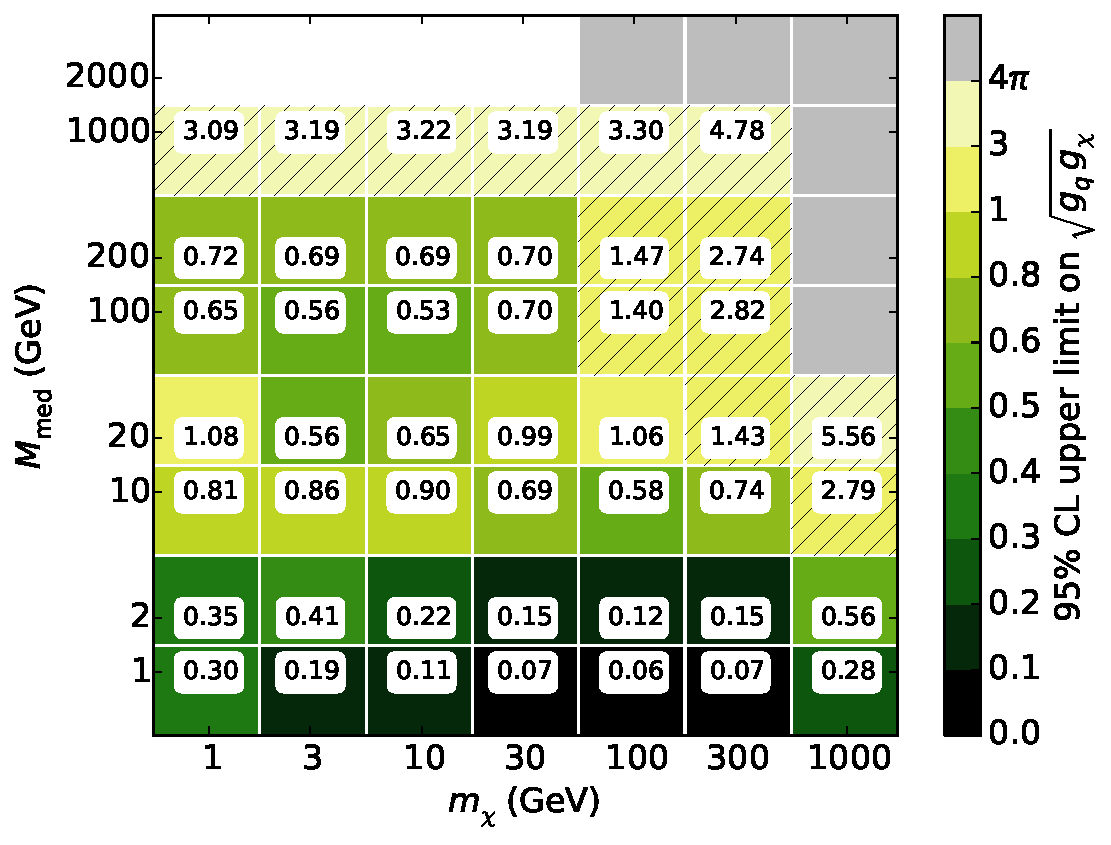
\includegraphics[width=1.\textwidth]{figures/grid_allpoints_SAD_rat1.pdf}
    \caption{sA model, $g_q/g_{\chi} = 0.5$, \monoZ channel.}
  \end{subfigure}
  \begin{subfigure}[t]{0.32\textwidth}
    \centering
    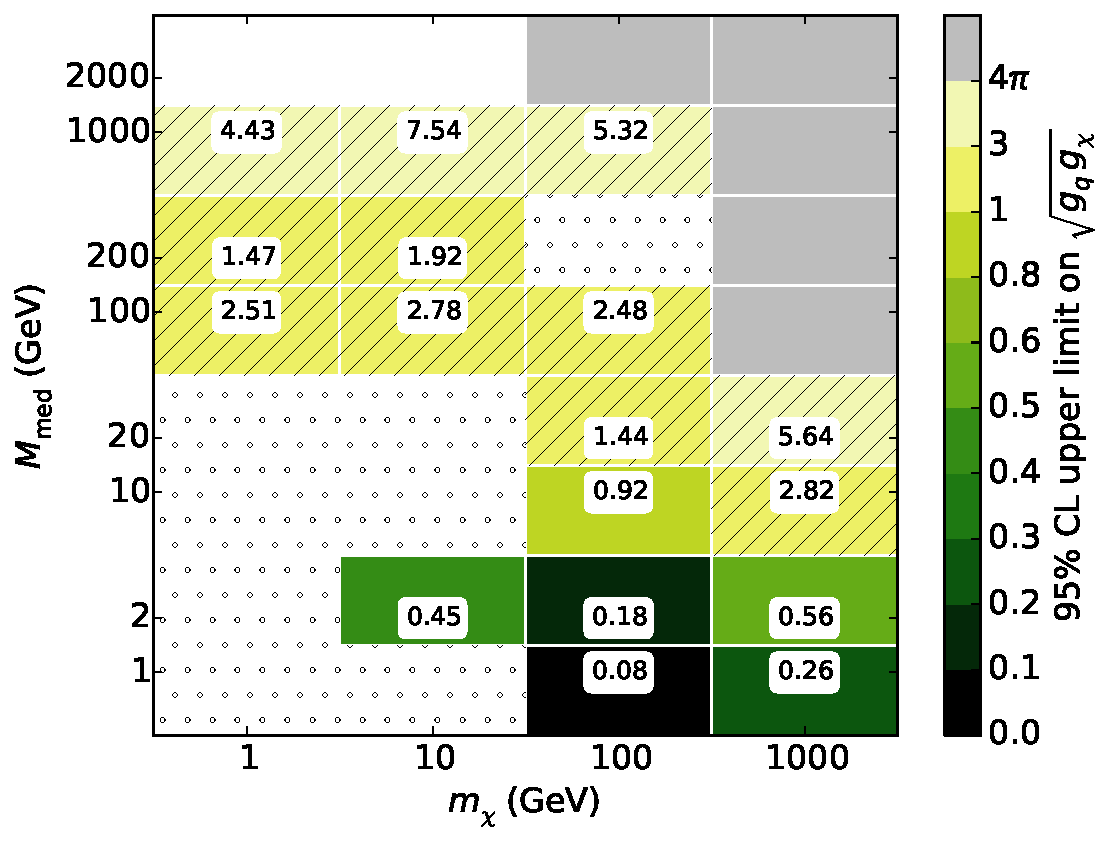
\includegraphics[width=1.\textwidth]{figures/grid_basepoints_SAD_rat1_monoWZ.pdf}
    \caption{sA model, $g_q/g_{\chi} = 0.5$, \monoWZ channel.}
  \end{subfigure}
  \caption{Upper limits on the couplings for the $s$-channel models in the \monojet (left), \monoZ (centre) and \monoWZ (right) channels, for $\gX / \gq$ = 1. Refer to fig.~\ref{fig:results_sVsA_rat05} for details.}
  \label{fig:results_sVsA_rat1}
\end{sidewaysfigure}

\begin{sidewaysfigure}
  \centering
  \begin{subfigure}[t]{0.32\textwidth}
    \centering
    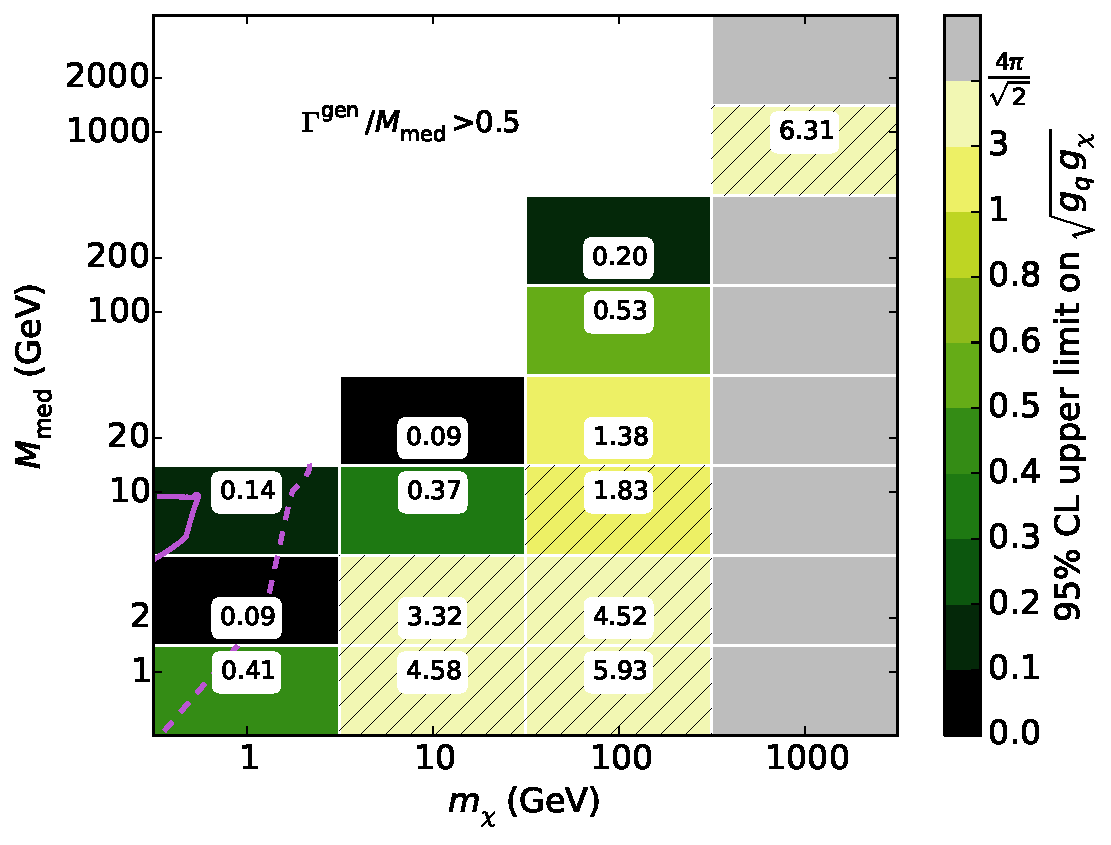
\includegraphics[width=1.\textwidth]{figures/grid_basepoints_SVD_rat2_monojet.pdf}
    \caption{sV model, $g_q/g_{\chi} = 0.5$, \monojet channel.}
  \end{subfigure}
  \begin{subfigure}[t]{0.32\textwidth}
    \centering
    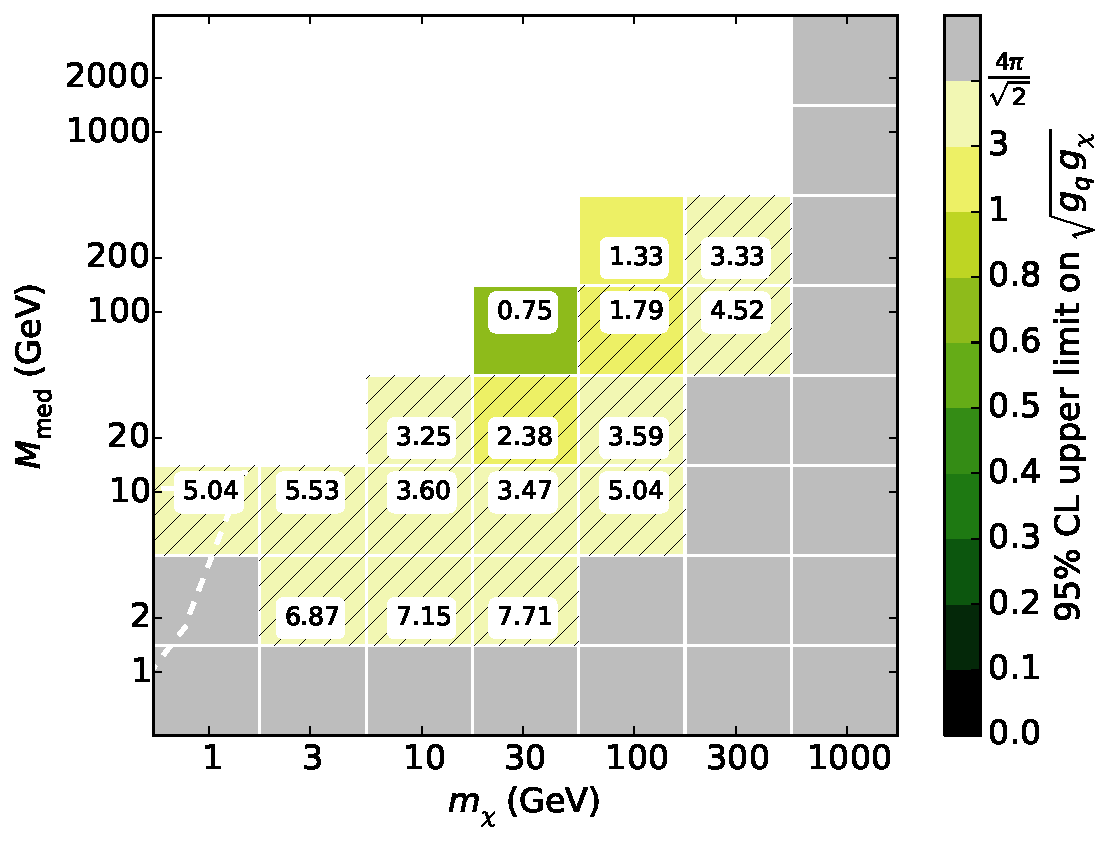
\includegraphics[width=1.\textwidth]{figures/grid_allpoints_SVD_rat2.pdf}
    \caption{sV model, $g_q/g_{\chi} = 0.5$, \monoZ channel.}
  \end{subfigure}
  \begin{subfigure}[t]{0.32\textwidth}
    \centering
    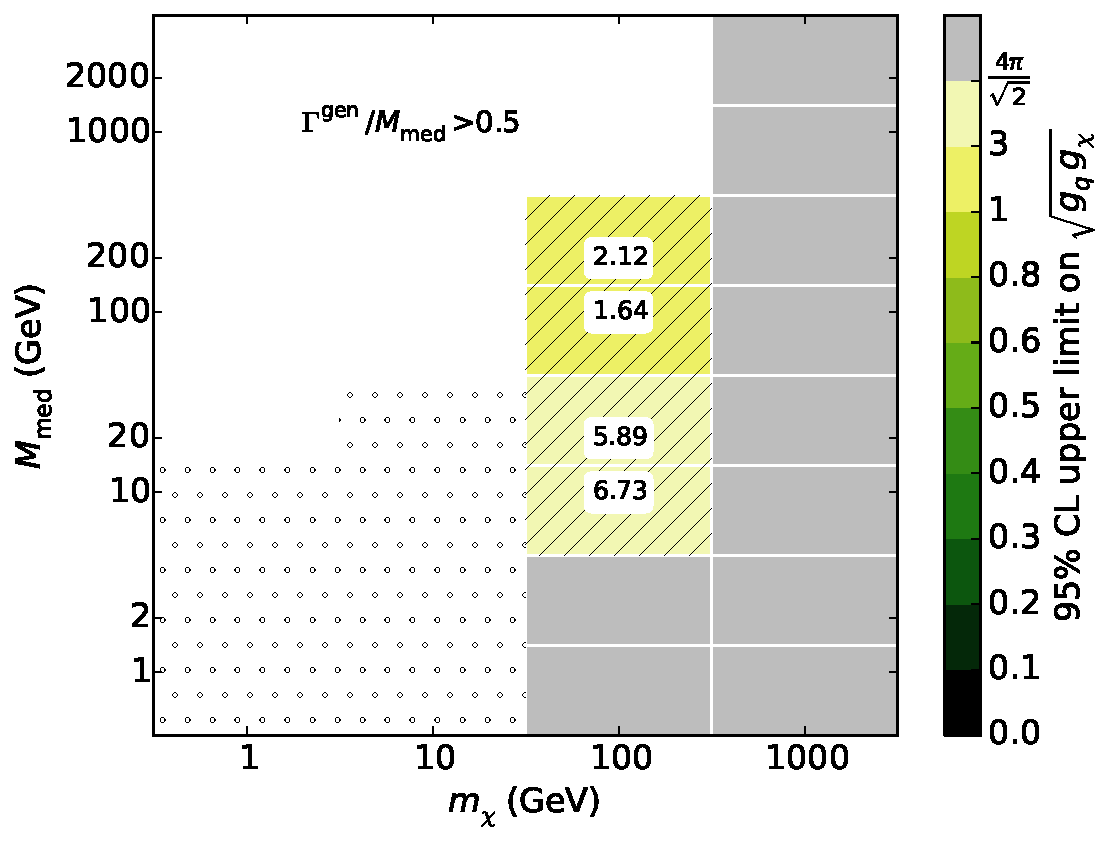
\includegraphics[width=1.\textwidth]{figures/grid_basepoints_SVD_rat2_monoWZ.pdf}
    \caption{sV model, $g_q/g_{\chi} = 0.5$, \monoWZ channel.}
    \vspace{0.75cm}
  \end{subfigure}
  \begin{subfigure}[t]{0.32\textwidth}
    \centering
    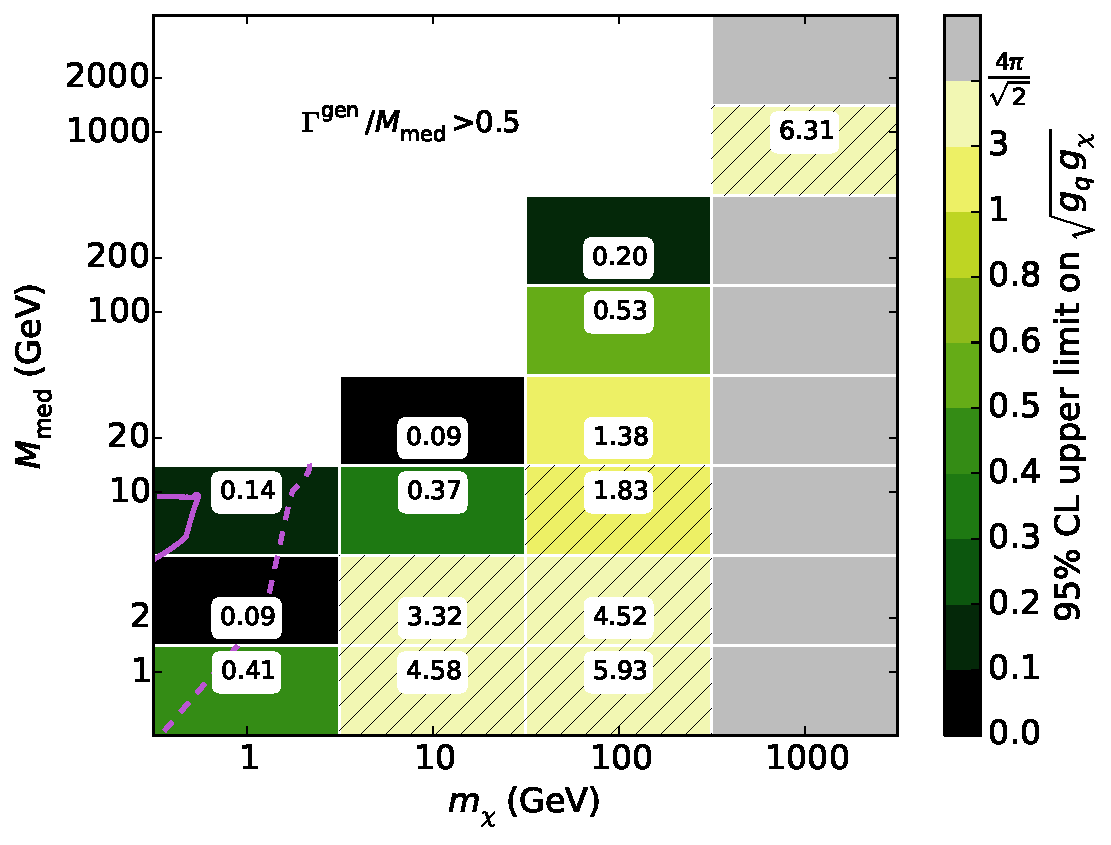
\includegraphics[width=1.\textwidth]{figures/grid_basepoints_SVD_rat2_monojet.pdf} % TODO change to SAD
    \caption{sA model, $g_q/g_{\chi} = 0.5$, \monojet channel.}
  \end{subfigure}
  \begin{subfigure}[t]{0.32\textwidth}
    \centering
    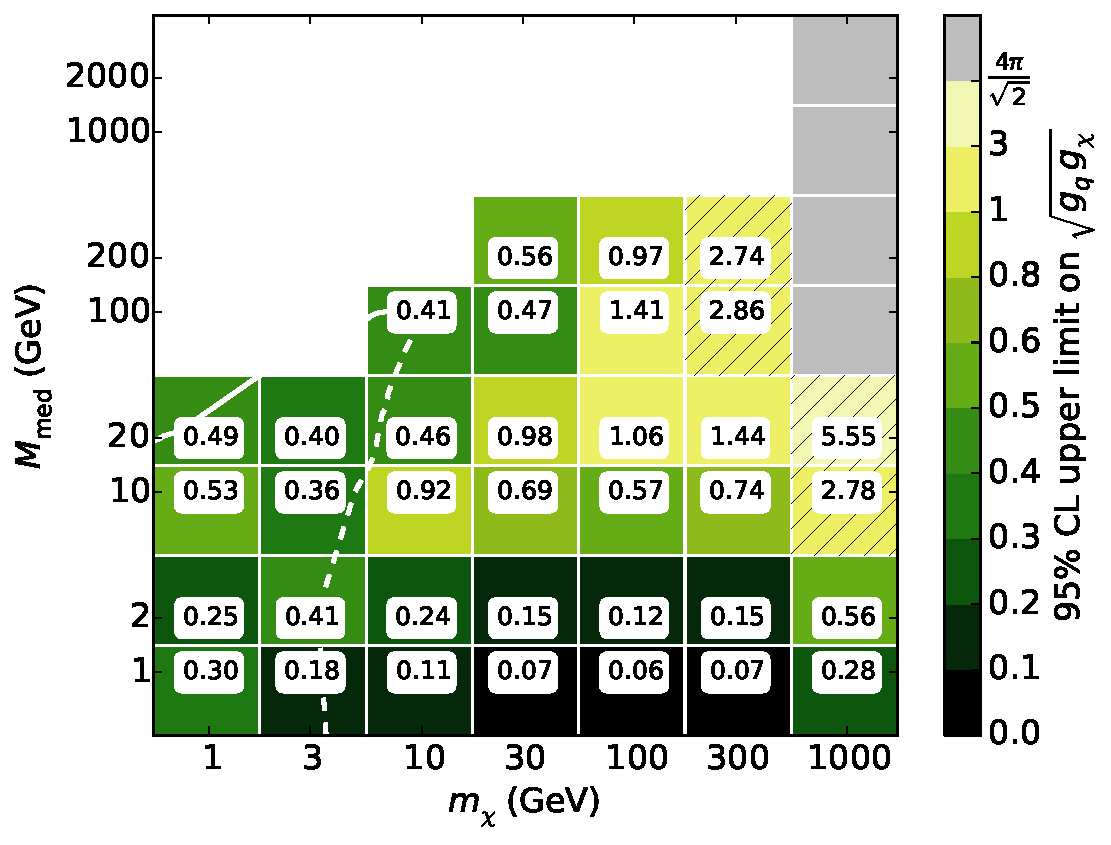
\includegraphics[width=1.\textwidth]{figures/grid_allpoints_SAD_rat2.pdf}
    \caption{sA model, $g_q/g_{\chi} = 0.5$, \monoZ channel.}
  \end{subfigure}
  \begin{subfigure}[t]{0.32\textwidth}
    \centering
    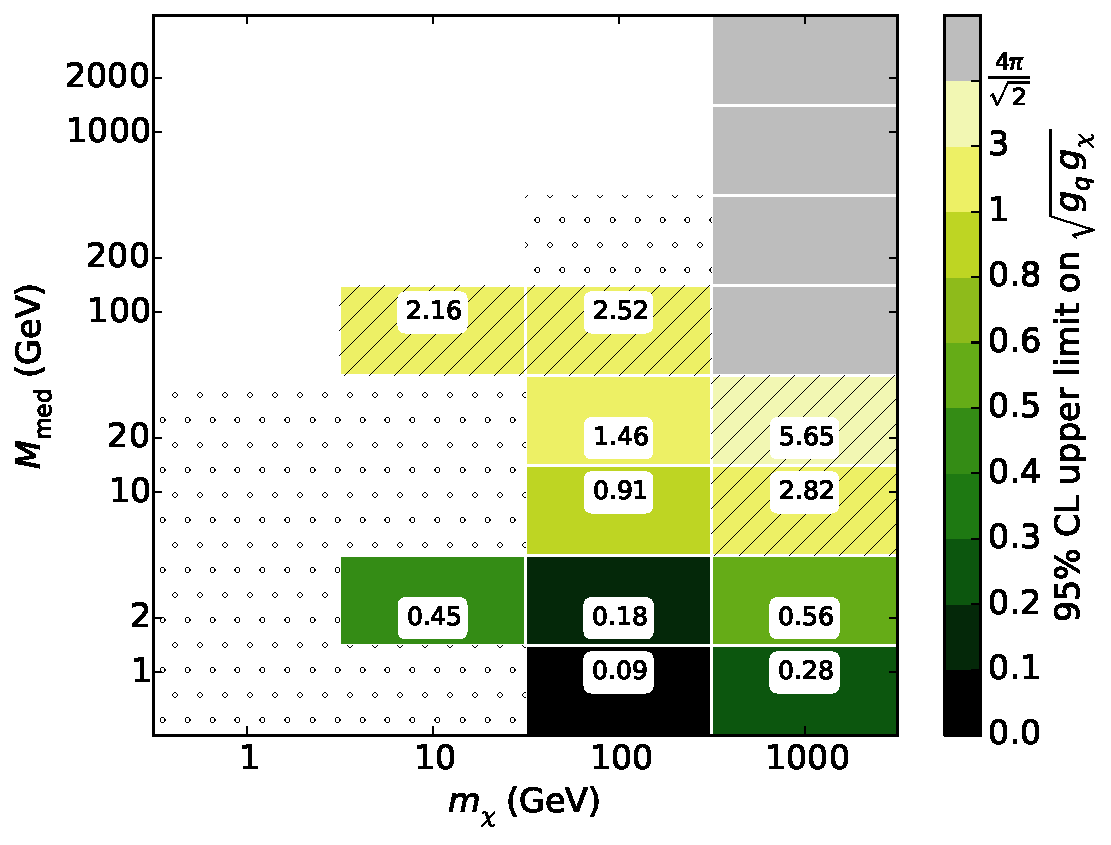
\includegraphics[width=1.\textwidth]{figures/grid_basepoints_SAD_rat2_monoWZ.pdf}
    \caption{sA model, $g_q/g_{\chi} = 0.5$, \monoWZ channel.}
  \end{subfigure}
  \caption{Upper limits on the coupling for the $s$-channel models in the \monojet (left), \monoZ (centre) and \monoWZ (right) channels, for $\gX / \gq$ = 2. Refer to fig.~\ref{fig:results_sVsA_rat05} for details.}
  \label{fig:results_sVsA_rat2}
\end{sidewaysfigure}

\begin{sidewaysfigure}
  \centering
  \begin{subfigure}[t]{0.32\textwidth}
    \centering
    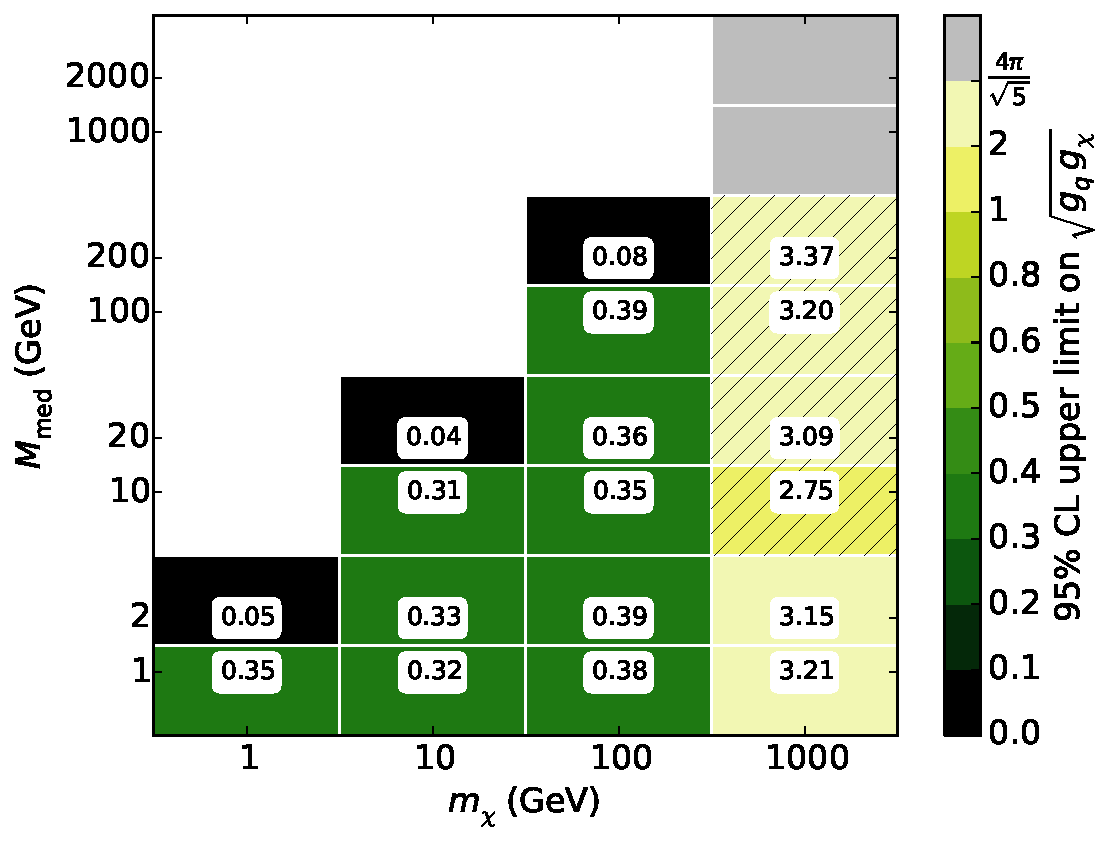
\includegraphics[width=1.\textwidth]{figures/grid_basepoints_SVD_rat5_monojet.pdf}
    \caption{sV model, $g_q/g_{\chi} = 0.5$, \monojet channel.}
  \end{subfigure}
  \begin{subfigure}[t]{0.32\textwidth}
    \centering
    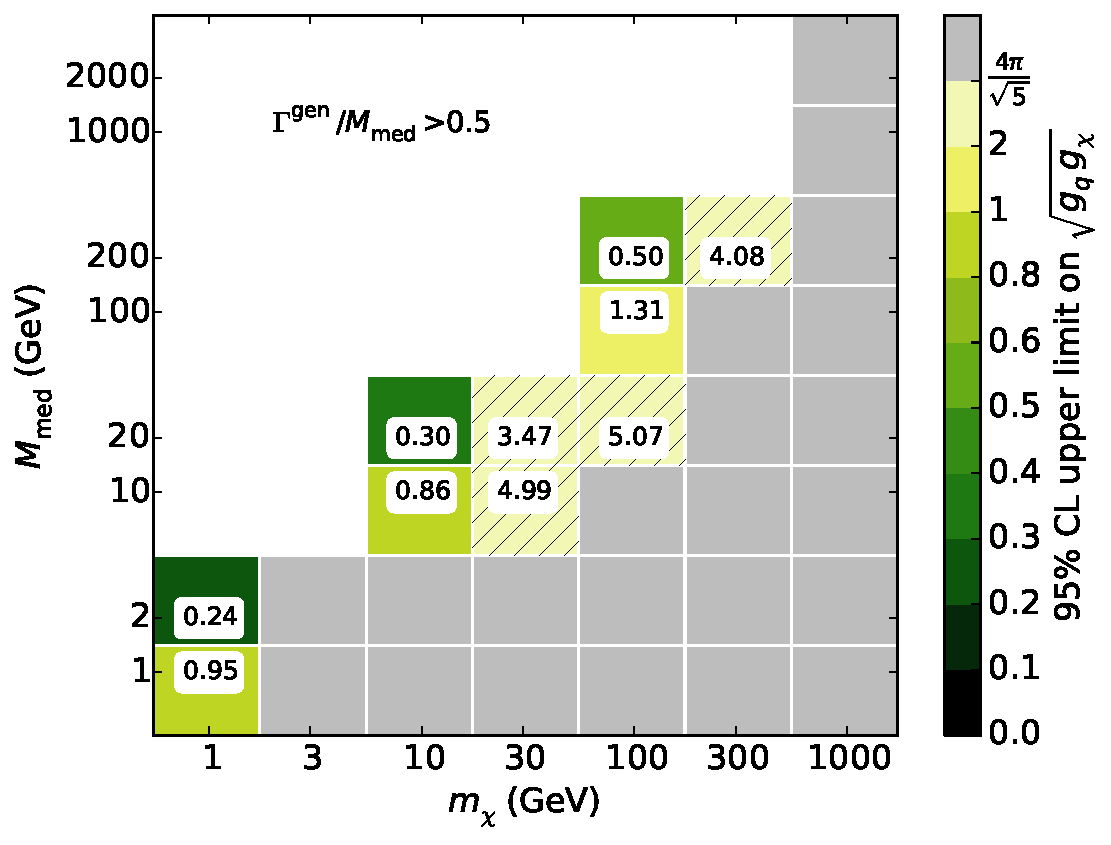
\includegraphics[width=1.\textwidth]{figures/grid_allpoints_SVD_rat5.pdf}
    \caption{sV model, $g_q/g_{\chi} = 0.5$, \monoZ channel.}
  \end{subfigure}
  \begin{subfigure}[t]{0.32\textwidth}
    \centering
    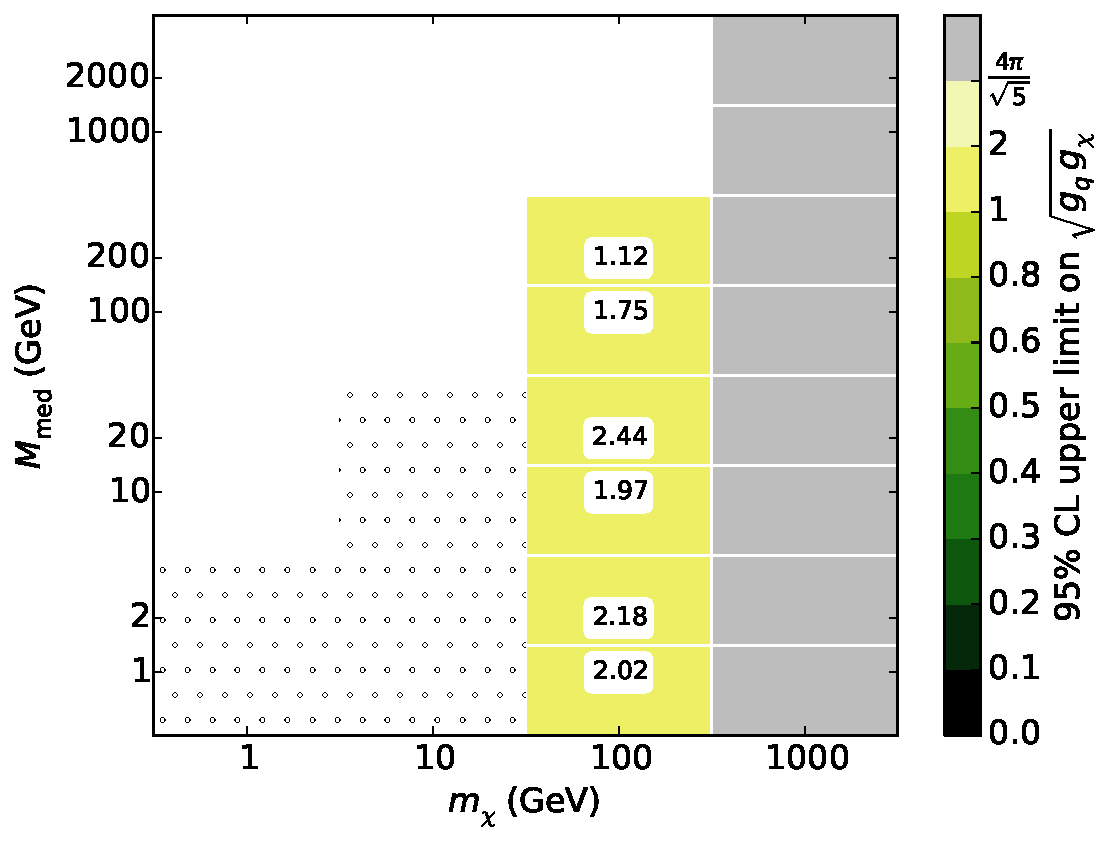
\includegraphics[width=1.\textwidth]{figures/grid_basepoints_SVD_rat5_monoWZ.pdf}
    \caption{sV model, $g_q/g_{\chi} = 0.5$, \monoWZ channel.}
    \vspace{0.75cm}
  \end{subfigure}
  \begin{subfigure}[t]{0.32\textwidth}
    \centering
    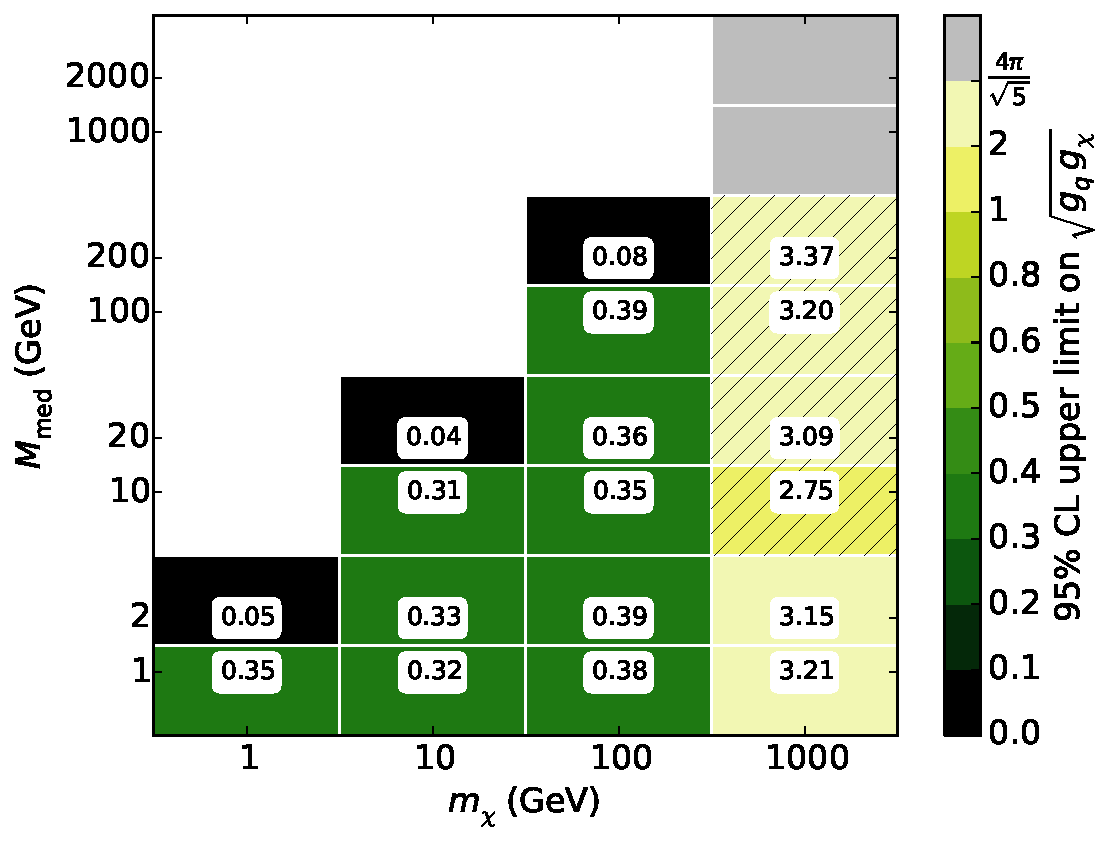
\includegraphics[width=1.\textwidth]{figures/grid_basepoints_SVD_rat5_monojet.pdf} % TODO change to SAD
    \caption{sA model, $g_q/g_{\chi} = 0.5$, \monojet channel.}
  \end{subfigure}
  \begin{subfigure}[t]{0.32\textwidth}
    \centering
    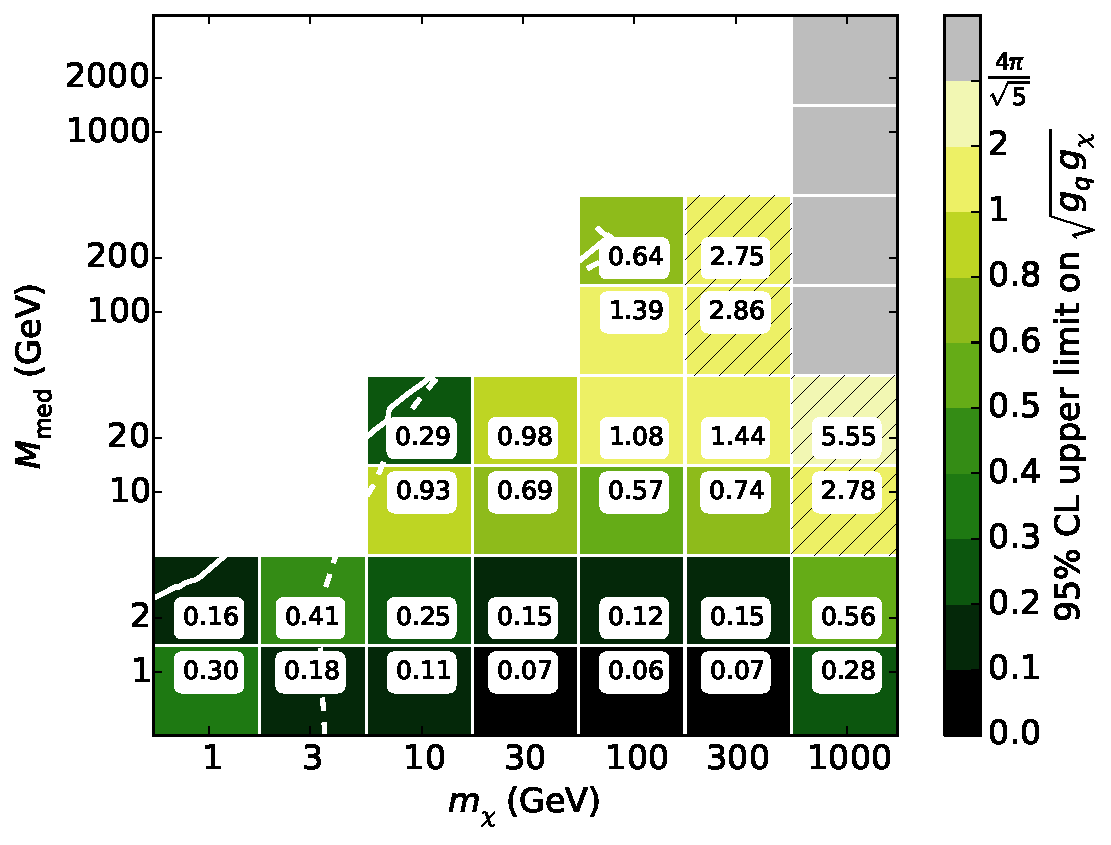
\includegraphics[width=1.\textwidth]{figures/grid_allpoints_SAD_rat5.pdf}
    \caption{sA model, $g_q/g_{\chi} = 0.5$, \monoZ channel.}
  \end{subfigure}
  \begin{subfigure}[t]{0.32\textwidth}
    \centering
    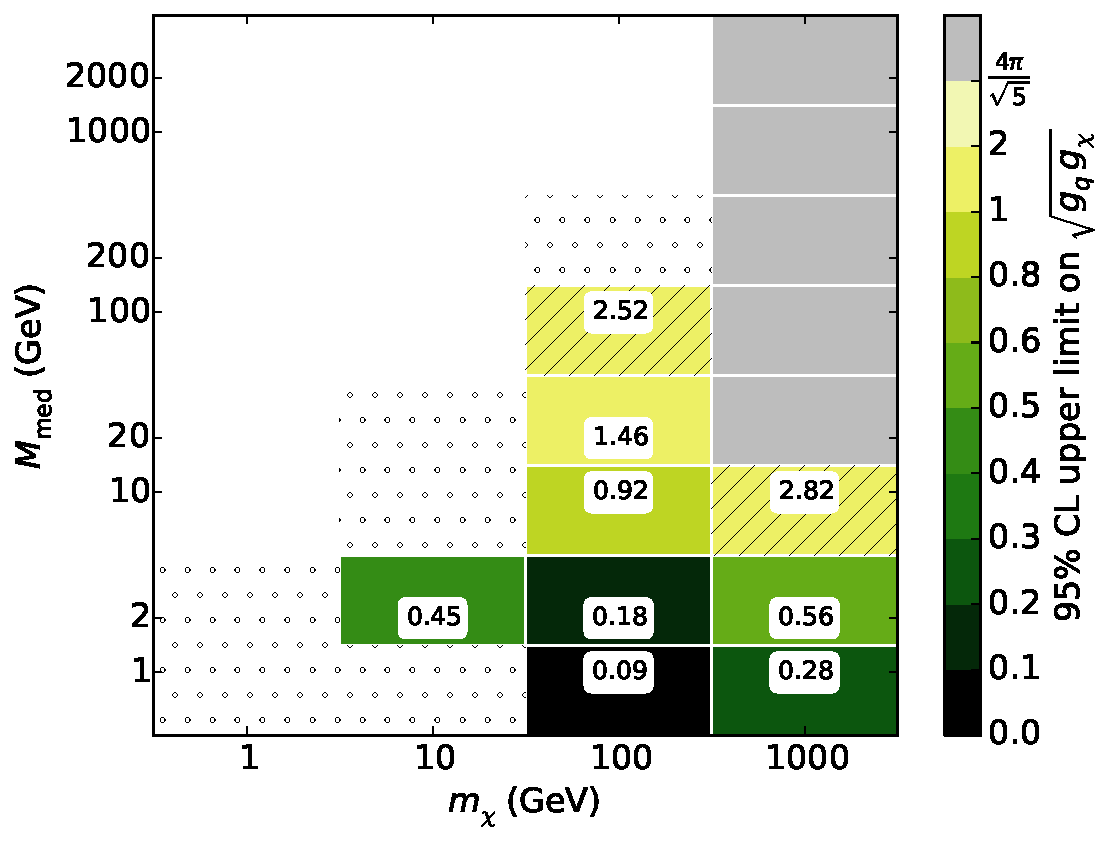
\includegraphics[width=1.\textwidth]{figures/grid_basepoints_SAD_rat5_monoWZ.pdf}
    \caption{sA model, $g_q/g_{\chi} = 0.5$, \monoWZ channel.}
  \end{subfigure}
  \caption{Upper limits on the coupling for the $s$-channel models in the \monojet (left), \monoZ (centre) and \monoWZ (right) channels, for $\gX / \gq$ = 5. Refer to fig.~\ref{fig:results_sVsA_rat05} for details.}
  \label{fig:results_sVsA_rat5}
\end{sidewaysfigure}

\begin{figure}
  \centering
  \begin{subfigure}[t]{0.495\textwidth}
    \centering
    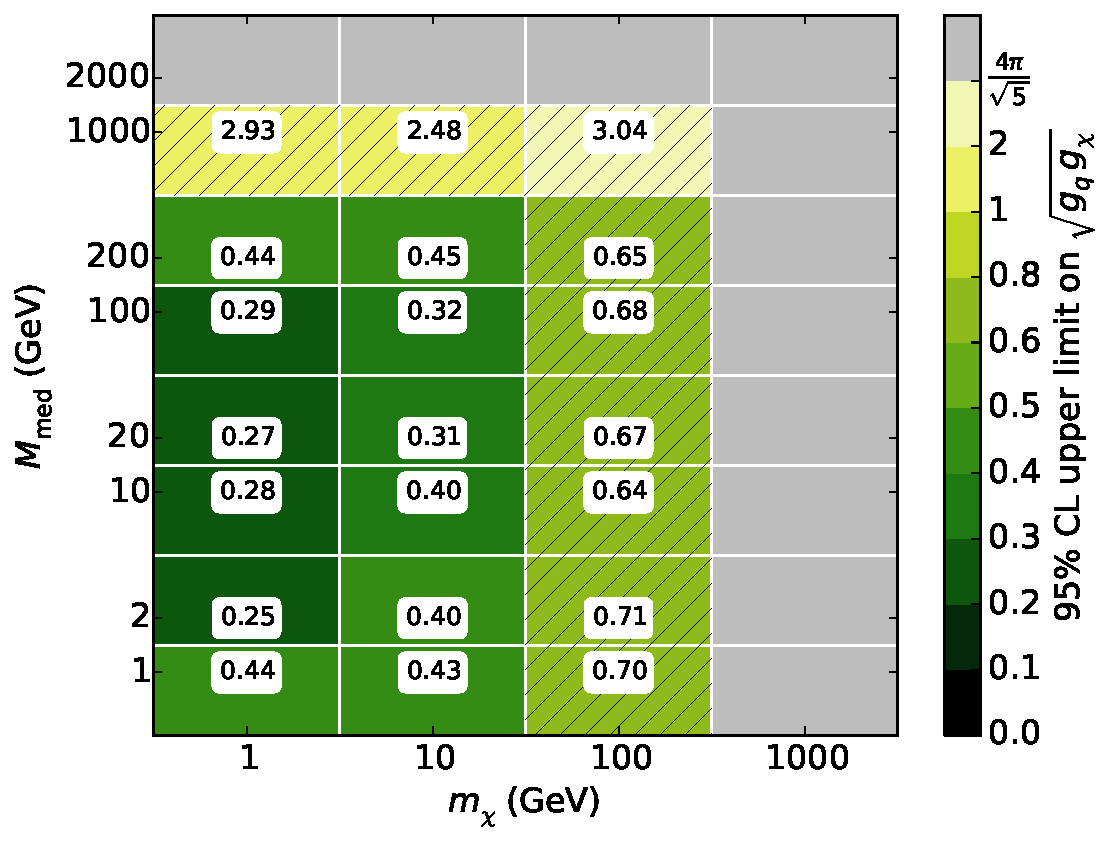
\includegraphics[width=1.\textwidth]{figures/grid_basepoints_SVD_rat02_monojet.pdf}
    \caption{sV model, $g_q/g_{\chi} = 0.2$, \monojet channel.}
  \end{subfigure}
  \begin{subfigure}[t]{0.495\textwidth}
    \centering
    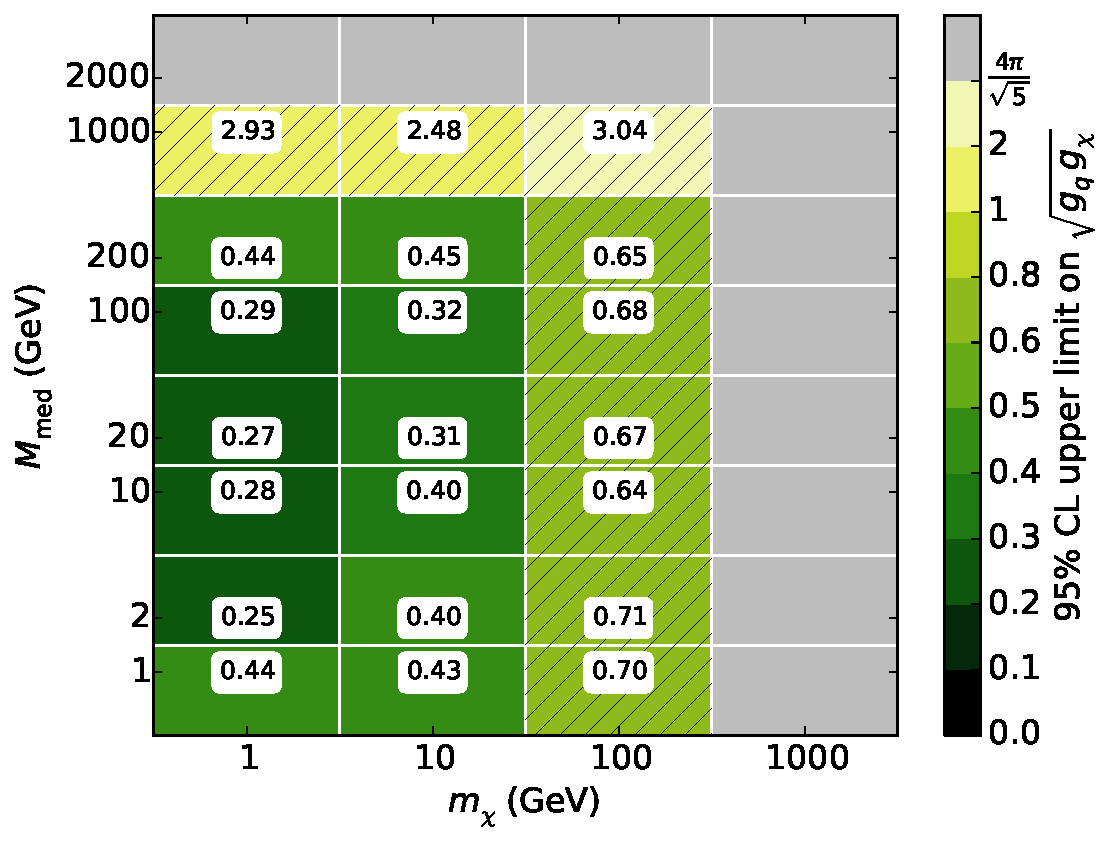
\includegraphics[width=1.\textwidth]{figures/grid_basepoints_SVD_rat02_monojet.pdf} % TODO change to SAD
    \caption{sA model, $g_q/g_{\chi} = 0.2$, \monojet channel.}
  \end{subfigure}
  \caption{Upper limits on the coupling for the $s$-channel models in the \monojet channel, for $\gX / \gq$ = 0.2. Refer to fig.~\ref{fig:results_sVsA_rat05} for details.}
  \label{fig:results_sVsA_rat02}
\end{figure}

\begin{figure}
  \centering
  \begin{subfigure}[t]{0.495\textwidth}
    \centering
    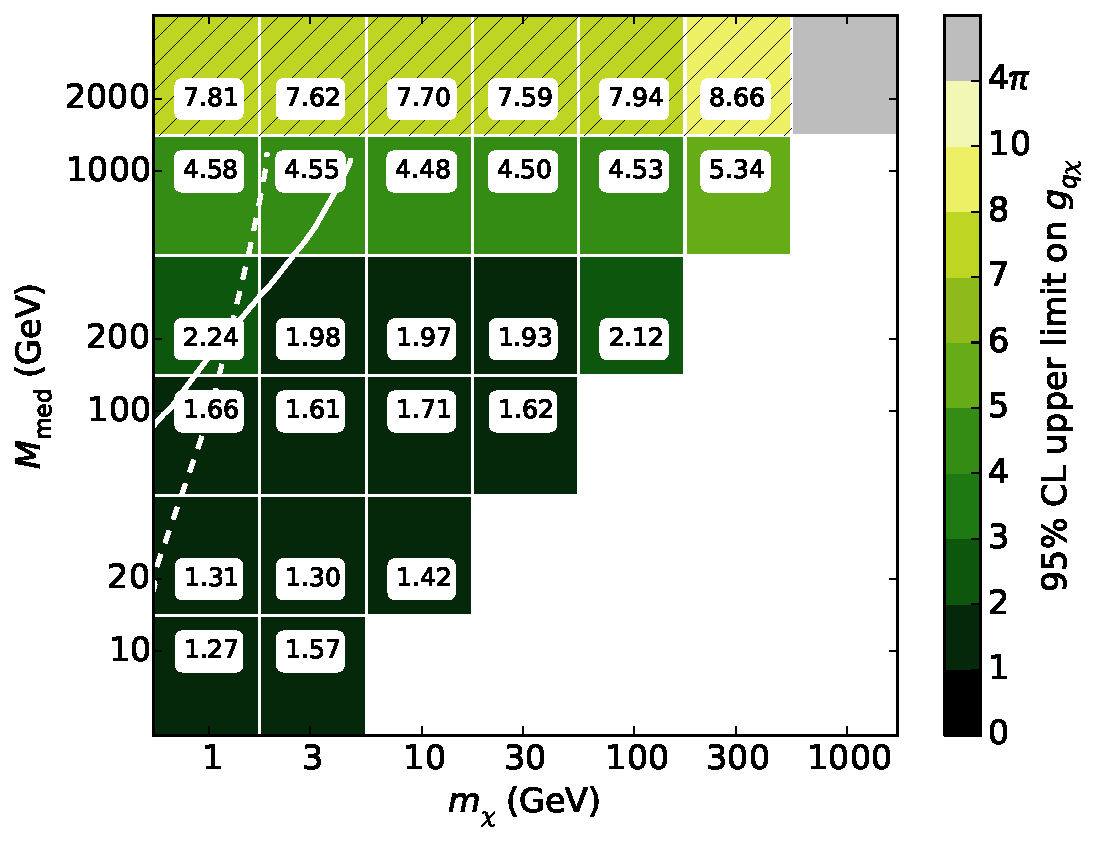
\includegraphics[width=1.\textwidth]{figures/grid_allpoints_TSD_rat1.pdf}
    \caption{tS model, \monoZ channel.}
  \end{subfigure}
  \begin{subfigure}[t]{0.495\textwidth}
    \centering
    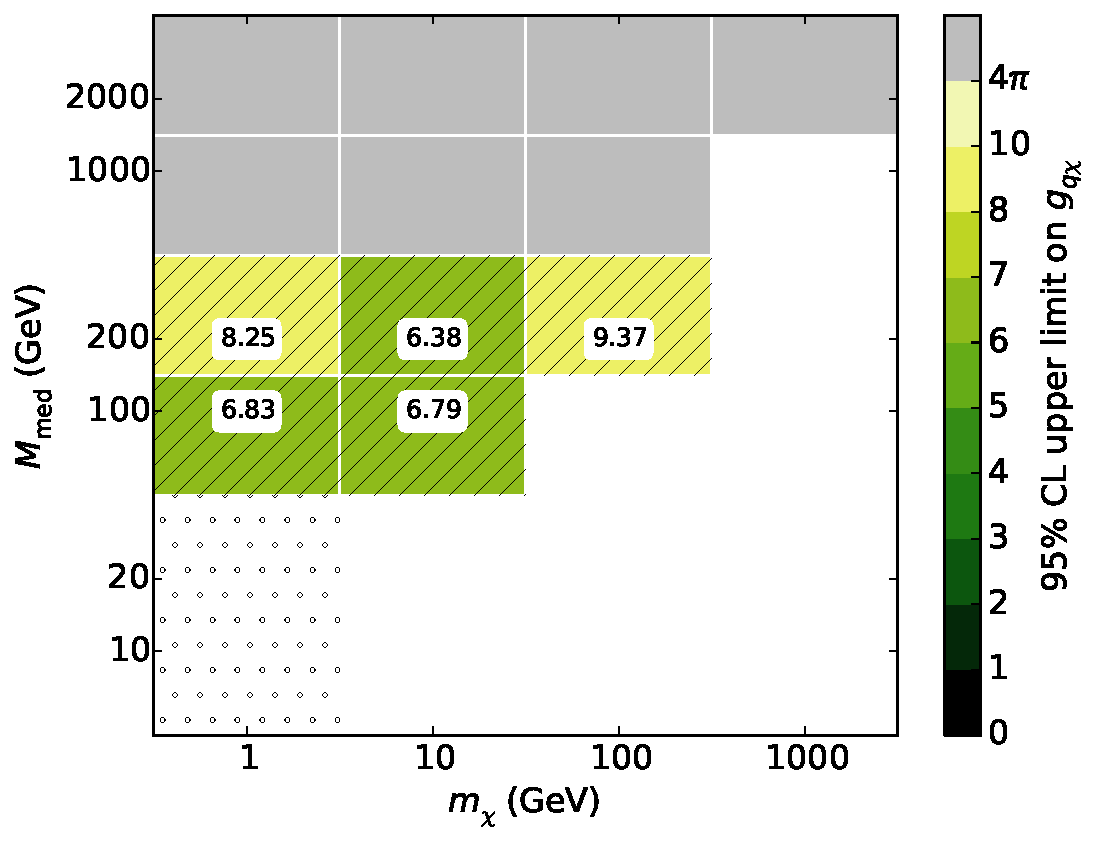
\includegraphics[width=1.\textwidth]{figures/grid_basepoints_TSD_rat1_monoWZ.pdf}
    \caption{tS model, \monoWZ channel.}
  \end{subfigure}
  \caption{Upper limits on the coupling $\gqX$ for the $t$-channel model in the \monoZ (left) and \monoWZ (right) channels. Refer to fig.~\ref{fig:results_sVsA_rat05} for details.}
  \label{fig:results_tS}
\end{figure}
